\section{Implementazione e descrizione dell'ambiente}\label{sec:Fault_Env}

\begin{figure}[h]
    \centering
    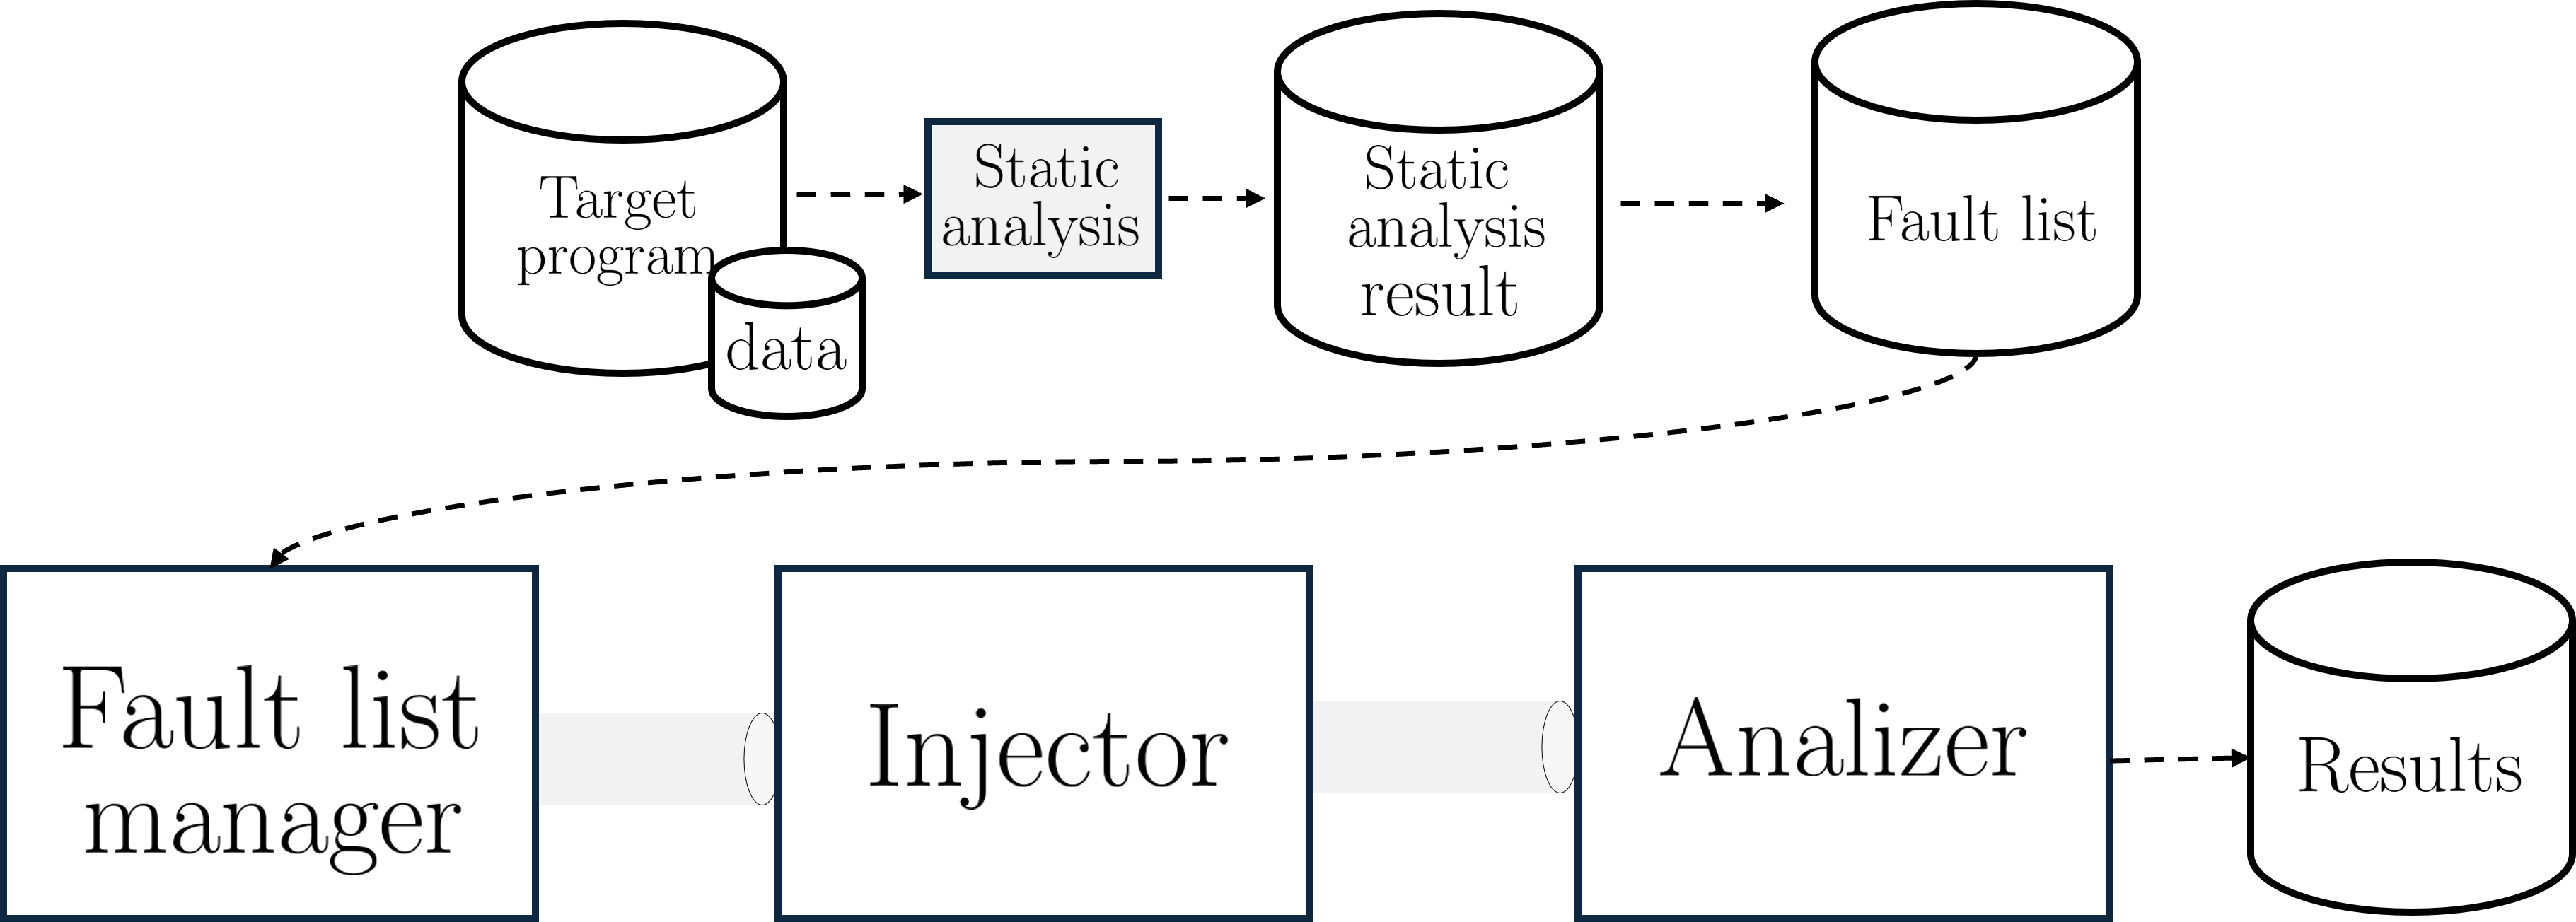
\includegraphics[scale=0.5]{img/pipeline.png}
    \caption{Struttura della pipeline}
\end{figure}

La fonte principale di ispirazione per la realizzazione della parte di applicazione devota ai fault injection è stato \cite{benso_fault_1998}.
Si possono individuare in questa parte principalmente tre sezioni: 
\begin{enumerate}
    \itemsep-0.3em
    \item \textsc{Fault List Manager} (FLM): genera la \textbf{lista dei fault} \textit{fault list} da iniettare nel \textbf{programma target}; 
    \item \textsc{Injector} \textit{(Fault injection Manager)} (FIM): \textbf{inietta i fault} nel programma target; 
    \item \textsc{Result Analyzer}: raccoglie i \textbf{risultati}, ne calcola degli \textbf{aggregati} e genera un \textbf{report} riferito al singolo esperimento di fault injection.
\end{enumerate}

Al fine di parallelizzare i compiti nei vari livelli si è deciso di adottare un \textit{pattern architetturale} che in letteratura è noto come \textbf{\textsc{pipes and filters}} (si veda il libro \cite{schmidt2013pattern} per una trattazione approfondita). Questo perché, come risulta evidente dall'introduzione, esistono nel progetto \textbf{fasi separate di elaborazione}. Inoltre tale struttura si presta molto bene allo sviluppo dell'applicativo in un team costituito da più persone. Per maggiore chiarezza dei concetti esposti si riporta qui una possibile definizione del pattern tratta da \cite{schmidt2013pattern}: 
\begin{quotation}
    \textit{
        \noindent
"The Pipes and Filters architectural pattern provides a structure for
systems that process a stream of \textbf{data}. Each processing step is
encapsulated in a \textbf{filter component}. Data is passed through \textbf{pipes}
between adjacent filters. Recombining filters allows you to build
families of related systems"}
\end{quotation}
Di seguito si riporta 
la versione modificata della pipeline in cui dove vengono aggiunti anche i componenti citati nella definizione. 

\begin{figure}[h]
    \centering
    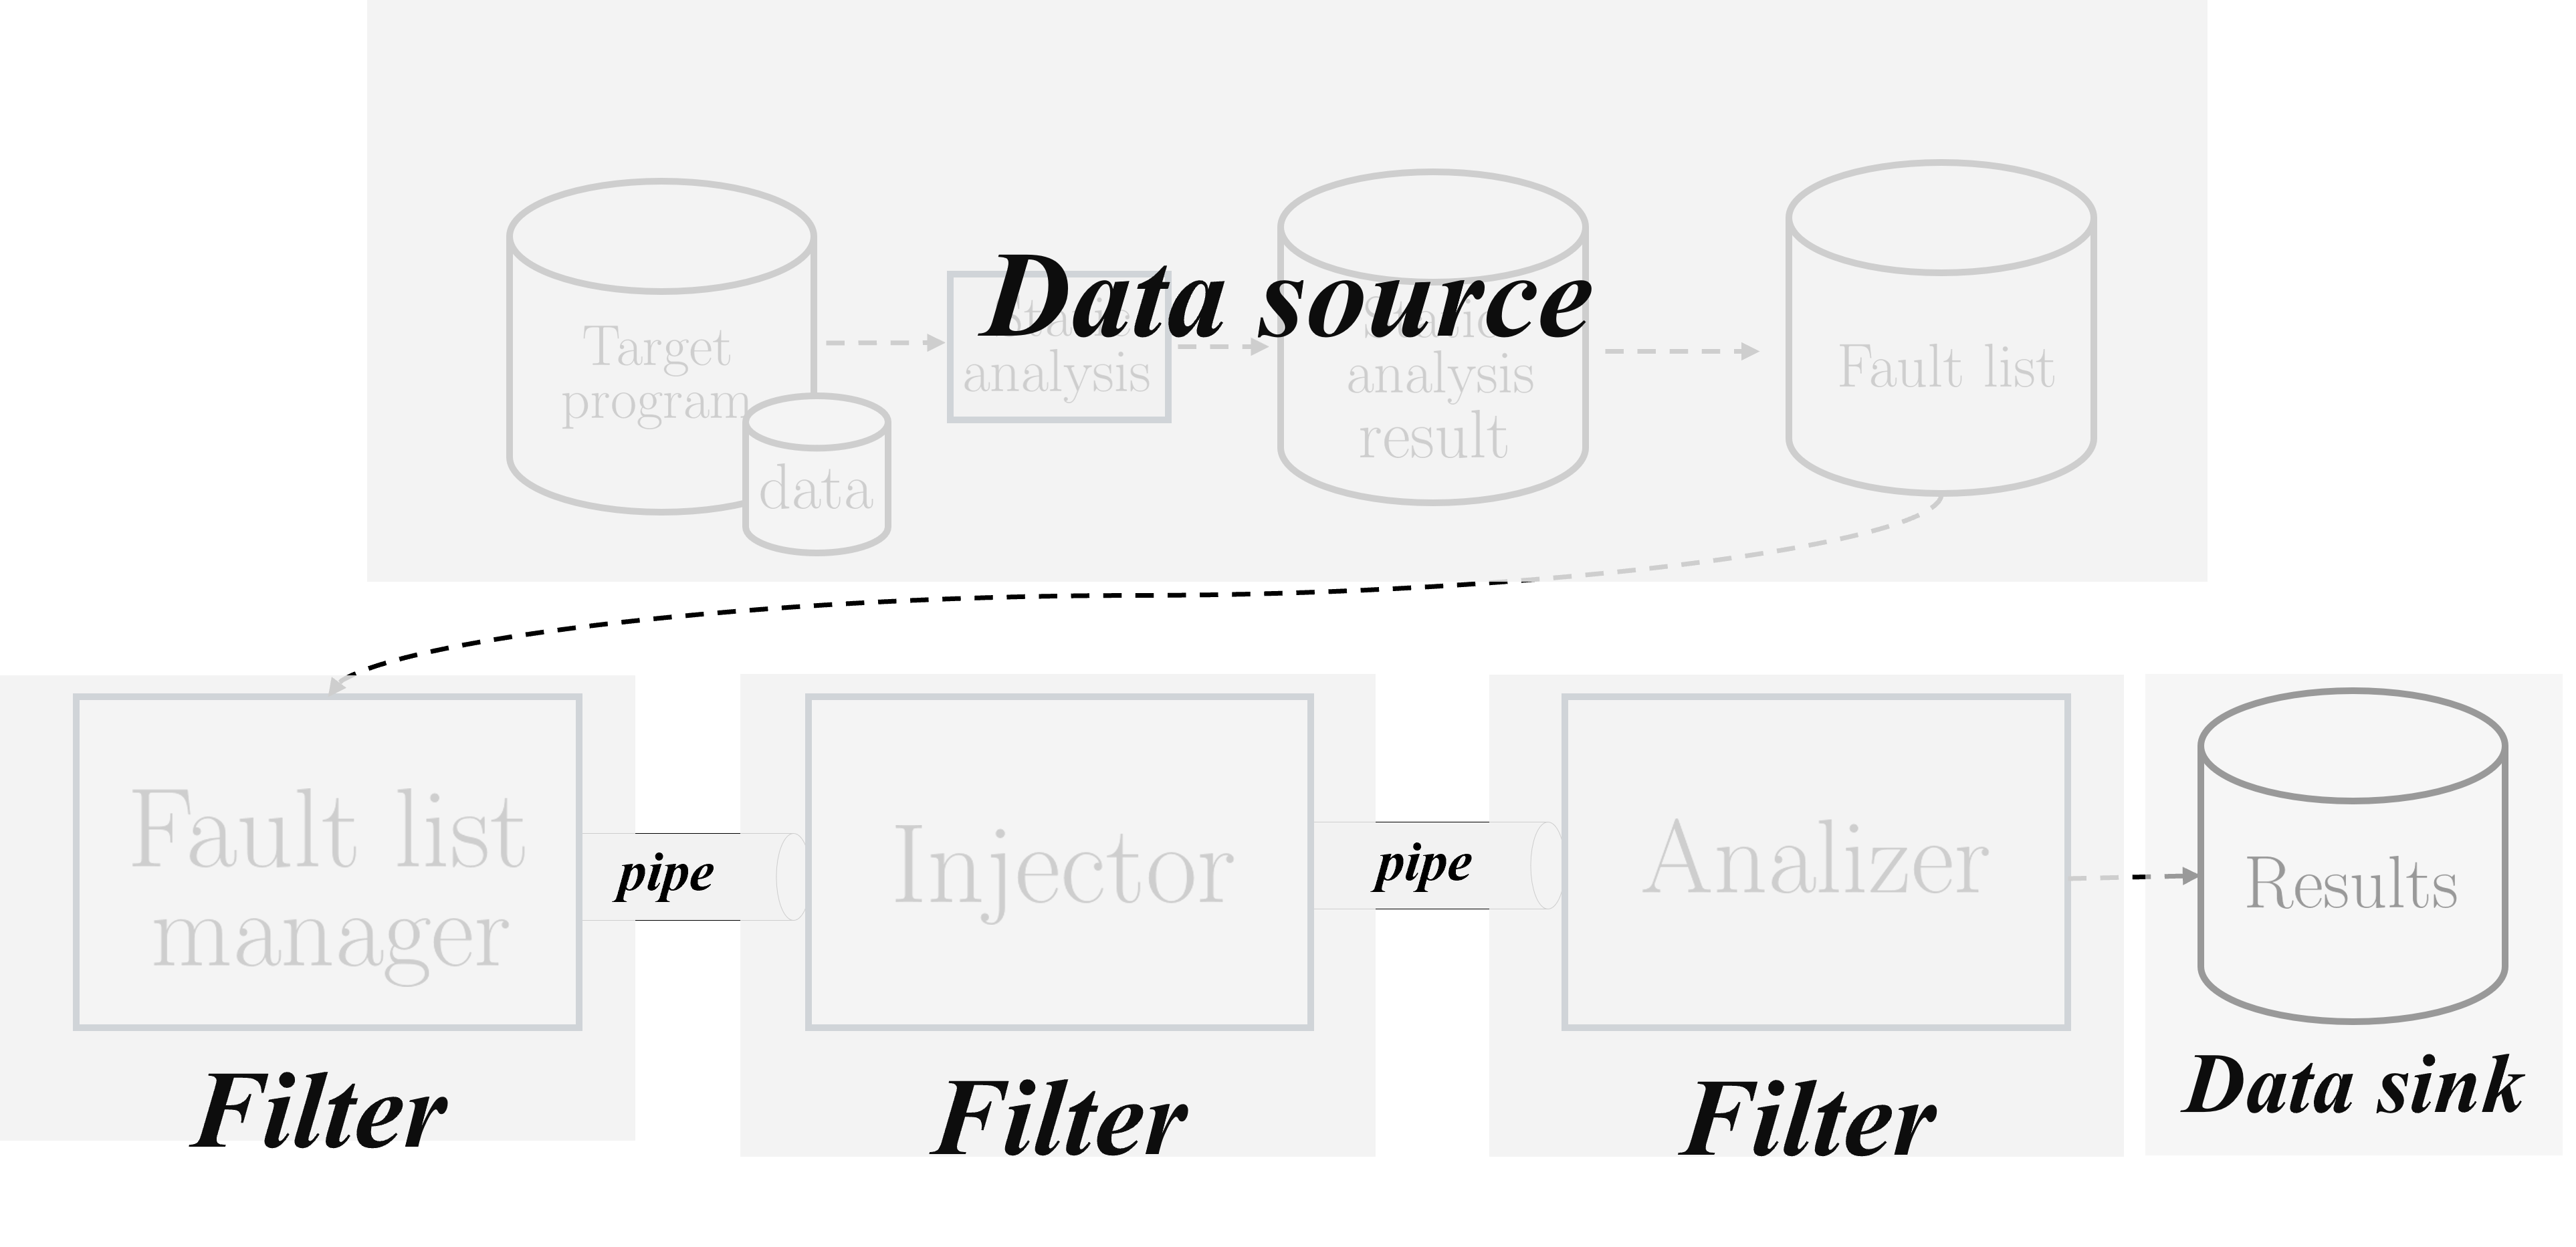
\includegraphics[scale=0.5]{img/pipeline_mapped.png}
    \caption{Pattern architetturale \textbf{pipes and filters}}
\end{figure}

\subsection{Implementazione in Rust}
Ogni componente della pipeline mostrata trova implementazione in Rust in opportuni componenti software. La \textsc{sorgente dei dati} è costituita da un sottosistema che esegue l'\textbf{analisi statica automatica} del \textbf{programma target} producendo un primo report (\textit{Static analysis result)} (data preparation) che viene utilizzato a sua volta da una routine preposta alla generazione della \textbf{generare la fault list}. I \textsc{tre filtri}, invece, sono delle subroutine allocate in appositi moduli. Le due \textsc{pipeline} tramite le quali comunicano i tre stage sono implementate tramite 2 canali \textit{multiple producer single consumer} \texttt{(mpsc)}. Ogni filtro\footnote{
    Questi in letteratura sono noti come \textit{filtri attivi} in quanto rispettano il seguente principio: "[...] the filter is active in a loop, pulling its input from
    and pushing its output down the pipeline."(cfr. \cite{schmidt2013pattern})
} utilizza come struttura di \textbf{programmazione concorrente} i thread.
In conclusione di questa sezione forniamo: (i) lo snippet di codice che riporta la \textbf{funzione di setup} della pipeline; una \textbf{tabella riassuntiva} (Tabella \ref{setup}) di tutti gli elementi della pipeline con annessa descrizione, ruolo e sezione di codice a cui afferisce.\newpage

\begin{lstlisting}[language=rust, style=boxed][h]
pub fn fault_injection_env(fault_list: String,   //Data Source: Fault List
                        target: String,          //Data Source: Target program
                        file_path: String,       //Data Sink: Report
                        data: Data<i32>) {       //Data Source: Data

    let (tx_chan_fm_inj, rx_chan_fm_inj) = channel();           //pipe FLM-FIM
    let (tx_chan_inj_anl, rx_chan_inj_anl) = channel();         //pipe FIM-Analyzer

    fault_manager(tx_chan_fm_inj,fault_list);
    injector_manager(rx_chan_fm_inj, tx_chan_inj_anl, target, data);
    analyzer(rx_chan_inj_anl,file_path);
}
\end{lstlisting}

\begin{table}[h] 
    \centering
    \small
    \begin{tabular}{p{4cm} p{2.5cm} p{8.5cm}}
        \toprule[1.5px]
        \textbf{\large Componente}&\textbf{\large Ruolo}&\textbf{\large Descrizione}\\
        \midrule[1.5px]
        \textsc{Static analysis result}&Data source&Dato il programma target lo analizza estrandone le informazioni sulle variabili (tipo, nome, dimensione...) ed  effettua un conteggio delle istruzioni. Il sottomodulo \texttt{mod static\_analysis} contiene tutte le funzioni collegate a questo task.\\
        \hline
        \textsc{Target program}&Data source&
            Codice sorgente dei casi di studio oggetto dell'analisi: irrobustimento dei dati e fault injection. La directory \texttt{fault\_list\_manager/file\_fault\_list} contiene i file \texttt{*.rs} input dell'analisi statica.\\
            \hline
            Data&Data source&Sono i dati su cui lavorano gli algoritmi selezionati come casi di studio. I dati possono essere prelevati dal file \texttt{data/input.txt} o dai dataset \texttt{data/dataset.txt}.\\
            \hline
        \textsc{Fault list}&Data source& Sfruttando il report prodotto dall'analisi statica viene generata la fault list contenente un numero di entry scelto dall'utente o prefissato. Il modulo \texttt{mod fault\_list\_manager} contiene le funzioni adibite a tale compito.\\
        \midrule
        \textsc{Fault list manager}&Filter&Stage della pipeline che scorre la fault list, preleva una fault entry per volta e la spedisce nella \textit{pipe} verso l'iniettore incapsulato in una struttura di tipo \texttt{FaultListEntry}. (\texttt{mod fault\_list\_manager})\\\hline
        \textsc{Injector}&Filter&Prelevando dal canale le \texttt{FaultListEntry} esegue gli esperimenti di iniezione e spedisce i risultati grezzi da analizzare a valle nella pipeline. \texttt{(mod injector)}\\\hline
        \textsc{Analizer}&Filter&Stage della pipeline che riceve i risultati dei test dall'iniettore, calcola delle statistiche e produce il report finale dell'esperimento. (\texttt{mod analizer})\\\hline
        \textsc{Results}&Data sinks&File contenente il report dell'esperimento di fault injection con grafici e tabelle. Viene memorizzato nella directory \texttt{result}.\\
        \midrule
        \textsc{Canali} \texttt{mpsc}&pipes&Costituiscono il collante degli stage della pipeline. Le istruzioni 6-7 creano le estremità delle due pipeline, queste vengono poi distribuite ai vari filtri.\\
        \bottomrule[1.5px]
   \end{tabular}
    \caption{Tabella riassuntiva \textit{Fault injection environment}}
    \label{setup}
\end{table}